\documentclass{article}

\usepackage{mathtools,amsfonts}
\usepackage{enumerate}
\usepackage{fullpage}
\usepackage{array}
\usepackage{fancyvrb}

\begin{document}
\thispagestyle{empty}

\begin{center}
  \textbf{\Large Beginner Test 1}
  % LEVEL is Senior, Intermediate or Beginner
  % NUMBER is the test number: 1, 2, etc.
  \\ \vspace{1em}
  \textbf{\large January Camp 2021}
  \\ \vspace{1em}
  \textbf{\large Time: $2\frac{1}{2}$ hours}
\end{center}

\vspace{24pt}

\begin{enumerate}[1.]


\item What is the ratio of the areas of the two squares given below:
\begin{center}
	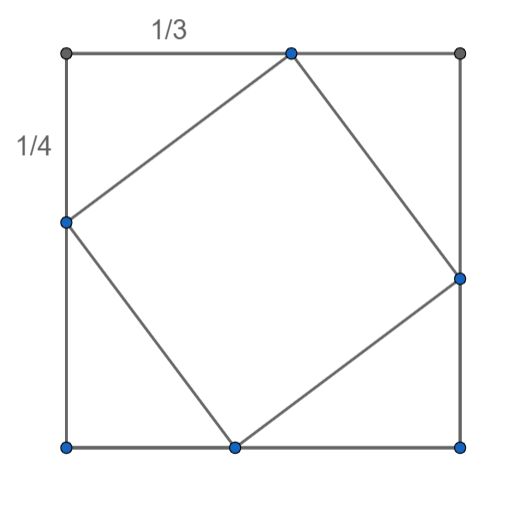
\includegraphics[scale=0.4]{beginner_test_1_img_2.png}	
\end{center}
Remember to prove your answer.\\% Tim

\textbf{Solution:}\\
The side of the smaller square, by Pythagoras: $\sqrt{(\frac{1}{4})^2+(\frac{1}{3})^2}=\frac{5}{12}$\\
The side of the larger square: $\frac{1}{3}+\frac{1}{4}=\frac{7}{12}$\\
The ratio of the areas of these squares: $(\frac{5}{12}/\frac{7}{12})^2=\frac{25}{49}$\\



\item Find, with proof, the smallest three different positive integers whose squares sum to the square of an integer.\\ % Tim

\textbf{Solution:}\\
We want the smallest $a,b,c$ with $a^2+b^2+c^2=d^2$. Assuming $c$ to be larger than $a$ and $b$ (W.L.O.G.), we have $a^2+b^2=d^2-c^2$. Looking at some of the smallest values for $a$ and $b$, we try $a=1$, $b=2$. A difference of 5 means $d=3$, $c=2$. But then $b=c$ when they must be different. We then try $a=1$, $b=3$. A difference of 10 between two squares is not possible. Now, we try $a=2$, $b=3$. A difference of 13 means $d=7$, $c=6$. Finally, we try $a=2$, $b=4$. A difference of 20 can be broken up into 9+11, so we get $c=4$, $d=6$. Again, $b=c$. Any other solution will clearly result in a larger triple, so we choose 2,3,6.\\



\item Find, with proof, 4 fractions strictly between $\frac{1}{3}$ and $\frac{1}{2}$ with denominator less than 10.\\ % Tim

\textbf{Solution:}\\
The fractions are $\frac{2}{5},\frac{3}{8},\frac{3}{7},\frac{4}{9}$. The check is left as an exercise.\\

\newpage

\item What fraction of the following shape is shaded:
\begin{center}
	
\includegraphics[scale=1.0]{beginner_test_1_img_1.png}	
\end{center}
Prove your answer.\\
\textit{Note: The dots are spaced evenly around the circle and the only interior point used is the center of the circle.}\\

% Catriona Shearer, https://mathwithbaddrawings.com/2018/10/03/twenty-questions-of-maddening-delicious-geometry/
\textbf{Solution:}\\
\begin{center}
	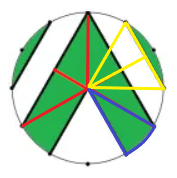
\includegraphics[scale=1.0]{beginner_test_1_sol_img_1.png}	
\end{center}
Note that the sketch is symmetric vertically and there are 12 dots. The blue segment and its counterpart each cover $\frac{1}{12}$ of the area. The red triangles can be rotated into the yellow triangles to form a segment on either side that each cover $\frac{2}{12}$ of the area. Altogether, this makes $\frac{6}{12}=\frac{1}{2}$.\\



\item You are given that T,W,O,N,E are all different digits from 1 to 9 such that T+O+N=6 and:
\begin{center}
	\begin{tabular}{m{1cm} m{0.5cm} m{0.5cm} m{0.5cm}}
		&T&E&N\\
		+&T&W&O\\
		\hline
		&O&N&E\\
		\hline
	\end{tabular}
\end{center}
Find, with proof, the values of T,W,O,N,E.\\

% Tim
\textbf{Solution:}\\
T+O+N=6, and they are all different, so they are 1, 2 and 3 in some order. T being 1, 2 or 3 makes O 2, 3, 4, 5, 6 or 7. So O is either 2 or 3. But then T must be 1. Then, of course, N must be 3 or 2. Since O and N are 2 and 3 in some order, E must be 5. Since E$>$N, we must carry 1 over to the leftmost column. So O is 3. Then, W must be 7. In summary: T=1,W=7,O=3,N=2,E=5.\\



\item Ralph and Phil are playing a game. They have R12 in a bank account and can only withdraw coins of values R1, R2 and R5. The winner is the player who withdraws the last coin. If Ralph starts and they then alternate withdrawing one coin each (with a value of their choice), who has the winning strategy and how can they win?\\
\textit{Note: A winning strategy must be able to beat any sequence of moves that the opposing player decides to make.}\\

\textbf{Solution:}
We present a strategy for Phil to use, based on the idea that if we always leave a multiple of 3 in the bank account, Ralph will never be able to withdraw all of the money:\\
1: We start with 12 rand.\\
2: Ralph takes 1,2 or 5 rand, leaving Phil with 11, 10 or 7.\\
3: Phil chooses to take 2 rand if Ralph took 1, 1 if he took 2, and 1 if he took 5, leaving us with either 9 or 6 rand.\\
4: Ralph could leave Phil with any of 8, 7, 4, 5 or 1 rand.\\
5: Phil reduces the 8 to 3, the 7 to 6, the 4 to 3, and takes the win for the 5 or 1.\\
6: Ralph could leave Phil with any of 1, 2, 4, 5 rand.\\
7: Phil wins on 1, 2 and 5. He takes 1 rand from the 4.\\
8: Ralph could leave Phil with 1 or 2 rand.\\
9: Phil wins.\\



\item You are given the following shape: % South Africa, Tim's Assorted Combinatorics Questions 2020, Q2 (7 marks)
\begin{center}
	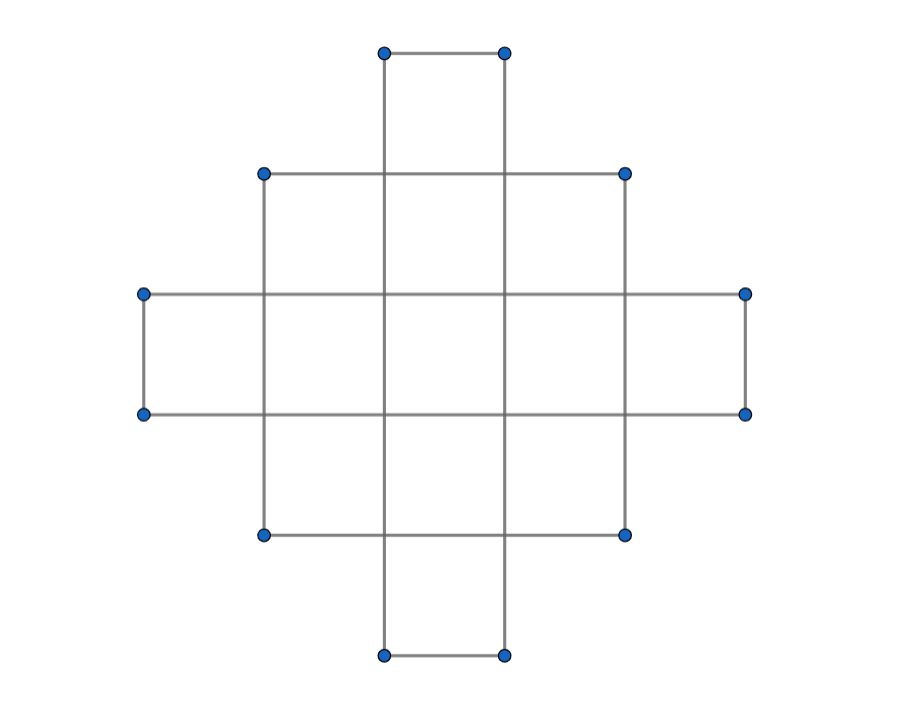
\includegraphics[scale=0.3]{Capture.png}	
\end{center}
	You need to tile this with L-shapes made of 3 blocks. Which single blocks could you shade out of the original diagram to make this possible?\\
	
\textbf{Solution:}\\
\begin{center}
	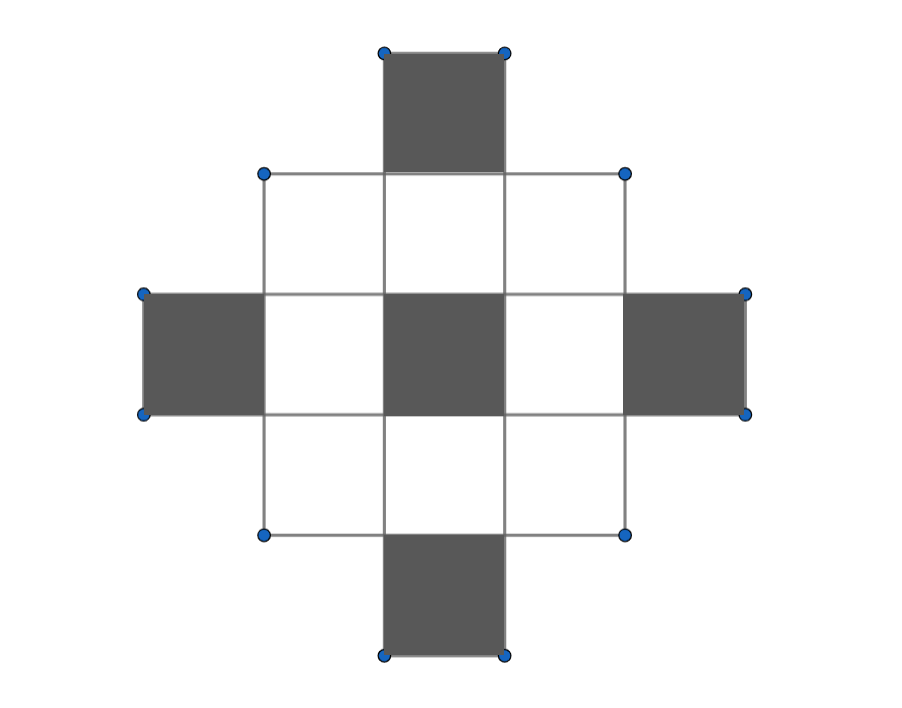
\includegraphics[scale=0.2]{beginner_test_1_sol_img_2.png}	
\end{center}
Note that any L-block covers at most 1 shaded square. To cover all of them, we would need 5 L-blocks, covering a total of 15 squares, when we only have 13 squares. So without removing one of these, we will not be able to tile the image. On the other hand, removing one of these squares always results in a possible tiling. This is left as an exercise.


\item % Moldova, 61st Maths Olympiad (2017), 7.1 modified
Find all natural numbers $x$, $y$ and $z$ satisfying 
$$x + \frac{1}{y + \frac{1}{z}} = \frac{850862}{421}$$\\

\textbf{Solution:}\\
Note $\frac{850862}{421}$ = $2021\frac{21}{421}$ where 2021 is the integer part of the fraction.

Since $y$ and $z$ are given as natural numbers, we have that $y + \frac{1}{z} > 1$ which implies $\frac{1}{y + \frac{1}{z}} < 1$. Since $x$ is a natural number,  $\frac{1}{y + \frac{1}{z}}$ will need to be the fractional part of  $2021\frac{21}{421}$. This will make $x$ the integer part of $2021\frac{21}{421}$ which means $x$ = 2021. Now we are left with $\frac{1}{y + \frac{1}{z}} = \frac{21}{421}$ which we can rewrite as $y + \frac{1}{z} = \frac{421}{21} = 20\frac{1}{21}$. Since $z\geq1$, we will have $\frac{1}{z}\leq1$. If $z = 1$, $y + \frac{1}{z} = y + \frac{1}{1} = y + 1 = 20\frac{1}{21}$ which would make $y = 19\frac{1}{21}$. This would be a contradiction since $y$ is given as a natural number. From this we conclude that $z\neq 1$ and that $\frac{1}{z}<1$ . This means that $\frac{1}{z}$ will be the fractional part and $y$ the integer part of $20\frac{1}{21}$. This makes $y = 20$ and $z = 21$. 
This means the only possible solution for $(x, y, z)$ is $(2021, 20, 21)$. 


\end{enumerate}


\vfill
% ASCII art
\centering
\begin{BVerbatim}
>o)
(_>
\end{BVerbatim}

\end{document}
